\documentclass[t]{beamer}
\setlength{\parskip}{5pt}
%\usetheme{Madrid}  

\usepackage[UKenglish]{babel}
\usepackage[UKenglish]{isodate}
\cleanlookdateon

%\usepackage{listings}
%\usepackage{tikz}
\usepackage{graphicx}

\newtheorem{remark}{Remark}

\def\le{\leqslant}
\def\ge{\geqslant}

\def\Z{\mathbb{Z}}
\def\N{\mathbb{N}}
\def\R{\mathbb{R}}
\def\C{\mathbb{C}}
\def\Q{\mathbb{Q}}

\title{CS3230 Tutorial 5}
\author{Deng Tianle (T15)}
\date{19 September 2025}

\begin{document}

\frame{\titlepage} 

\begin{frame}{Q1}
  Recall Freivald's algorithm: given $n \times n$ matrices $A, B, C$, we want to check whether $AB=C$. Choose a vector $v$ with components $\in \{0, 1\}$ randomly and check whether $ABv=Cv$. We proved in lecture that if $AB \ne C$, then $ABv \ne Cv$ (therefore, we successfuly detected $AB \ne C$) with probability $\ge 1/2$. 
  \par Q1: show that the bound is sharp, i.e. find $A, B, C$ such that the above probability is exactly $1/2$. 
  \pause
  \par Let $A=C=(1), B=(0)$. We have $AB \ne C$. We have $v = (v_1)$ where $v_1=0$ or $1$ with equal probability. Hence the above probability is $1/2$. It is easy to generalise the construction to $n \times n$ matrices. 
\end{frame}
\begin{frame}{Q2, 3}
  Alice holds an $n-$bit binary string $S_A \in \{0, 1\}^n$ and Bob holds an $n-$bit binary string $S_B \in \{0, 1\}^n$. They want to decide whether the two strings are identical i.e. $S_A = S_B$. 
  \par Q3: Obviously, to conclude deterministically that the $S_A = S_B$, all $n$ bits must be communicated.
  \par In Q2, We consider a randomised algorithm that only communicates $O(\log{n})$ bits. We show Q2 first before explaining the design of the algorithm. 
\end{frame}
\begin{frame}{Q2}
  We show that the probability of concluding wrongly is $\le 1/n$. 
  \par Observe that we are wrong iff $S_A \ne S_B$ but $S_A \equiv S_B \pmod{p}$, i.e. $p \mid |S_A-S_B|$. Note that $0 \le S_A, S_B < 2^n$, so $|S_A-S_B|<2^n$. 
  \par The number of choices of $p$ making us wrong is exactly the number of distinct prime factors of $|S_A-S_B|$. Since $p \ge 2$ for all prime $p$, there are at most $n-1$ prime factors. 
  \par Since we are choosing among $n^2$ different primes, probability of being wrong is $\le \frac{n-1}{n^2} \le \frac{1}{n}$.
\end{frame}
\begin{frame}
  Some explanations of the context:
  \begin{itemize}
    \item The reason we chose $n^2$ primes is seen in the preivous slide. 
    \item If we did not choose only primes but allow other numbers, we do not get an effective bound on the number of choices making us wrong.
    \item What is the size of the $n^2$th prime? According to the prime number theorem, the size of the $n$-th prime number is $\Theta(n \log{n})$. Therefore, in our case, $p \in \Theta(n^2 \log{n})$ and hence we are communicating $\Theta(\log(n^2 \log{n}))= \Theta(\log{n})$ many bits (this is in the tutorial document).
  \end{itemize}
\end{frame}
\begin{frame}{Q4}
  Let $X$ be the number of edges crossing $V_1$ and $V_2$. Let $X_e$ be the indicator random variable $\mathbf{1}_\text{$e$ crosses $V_1$ and $V_2$}$. Then
  \[X = \sum_{e \in E} X_e. \]
  Note that $\mathbb{E}(X_e) = \Pr(\text{$e$ crosses $V_1$ and $V_2$}) = 1/2$. Hence by linearity of expectation, 
  \[\mathbb{E}(X) = \sum_{e \in E} \mathbb{E}(X_e) = \sum_{e \in E} 1/2= |E|/2.\]
  %$\mathbf{1}$. $\Pr(\text{test})$. $\mathbb{E}(X)$
\end{frame}
\begin{frame}{Probabilistic method}
  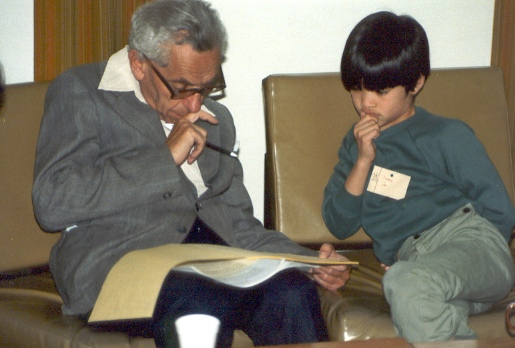
\includegraphics[scale=0.35]{Paul_Erdos_with_Terence_Tao.jpg}
  \par Let $X$ be some number we are interested in. In this case, $X$ is the size of a cut (a cut is a partition of the vertices of a graph into $V = V_1 \sqcup V_2$; size of the cut is the number of edges crossing $V_1$ and $V_2$). 
  \par If we turn $X$ into a random variable (with any distribution), then obviously there exists a configuration for which $X \ge \mathbb{E}(X)$. 
  \par This is a powerful method in combinatorics pioneered by Paul Erd\H{o}s called the probabilistic method. A magic of combinatorics is to solve deep problems using very simple ideas. 
\end{frame}
\begin{frame}{Q5}
  In Q4, we turned $X$ into a random variable by flipping a coin for each vertex, and obtained $\mathbb{E}(X) = |E|/2$ for the resulting distribution. This shows that any graph can admit a cut of size at least $|E|/2$. 
  \par Q5: Is there a way to tweak our distribution to get a higher $\mathbb{E}(X)$? 
  \par Let's first see how far the lower bound $|E|/2$ is from being attained. Subsequently, denote $n := |V|$ and $m := |E|$. For $K_n$, the complete graph with $n$ vertices, $m = n(n-1)/2$. If $n$ is even, we divde $V$ into half and obtain a cut with size $(n/2)^2$ which is slightly larger than $m/2$. If $n$ is odd, then we get a cut with size $\frac{n^2-1}{2}$. 
\end{frame}
\begin{frame}{Q5}
  Intuition: on average, it seems plausible that we will get a larger size of cut if $V_1$ and $V_2$ are approximately the same size. This suggests the following random procedure:
  \par Let $n$ be even. Choose $V_1$ uniformly at random from the collection of $n/2-$vertex subsets of $V$ and setting $V_2 = V-V_1$. Then we claim that 
  \[\mathbb{E}(X_e) = \Pr(\text{$e$ crosses $V_1$ and $V_2$}) = \frac{n/2}{n-1}. \]
  Indeed, fix a vertex of $e$ (WLOG let $e \in V_1$) and consider the other end of $e$, which is equally likely to be any of $n-1$ other vertices. Among them, $n/2$ vertices will be in $V_2$. 
  \par This gives
  \[\mathbb{E}(X) = \sum_{e \in E} \mathbb{E}(X_e) = m \cdot \frac{n/2}{n-1} = \frac{m}{2} \cdot \frac{n}{n-1}. \]
  It is clear that this lower bound is attained by our example with $K_n$. 
\end{frame}
\begin{frame}{Q5}
  The case $n$ is odd is similar, but $V_1, V_2$ will not have the same size. Let $|V_1| = \frac{n+1}{2}$. Then we condition on whether our fixed vertex is in $V_1$ or $V_2$:
  \[\mathbb{E}(X_e)= \frac{\frac{n-1}{2}}{n}\cdot \frac{\frac{n+1}{2}}{n-1} + \frac{\frac{n+1}{2}}{n}\cdot \frac{\frac{n-1}{2}}{n-1} = \frac{\frac{n+1}{2}}{n}.\]
  Hence
  \[\mathbb{E}(X) = m \cdot \frac{\frac{n+1}{2}}{n}= \frac{m}{2} \cdot \frac{n+1}{n}. \]
  Again this lower bound is attained by our example with $K_n$. 
\end{frame}
\end{document}
